\chapter{Revisão Bibliográfica} \label{cap:revisao}

\graphicspath{\currfiledir/figuras/} % caminho para as figuras deste capítulo

Este capítulo apresenta uma revisão da literatura sobre \textit{bots}, seu uso
em contextos educacionais e as tecnologias relacionadas ao seu desenvolvimento,
estabelecendo as bases conceituais para este trabalho.

O Capítulo está organizado da seguinte forma: a Seção \ref{sec:def-bots}
apresenta a definição e os componentes de \textit{bots}, a Seção
\ref{sec:class-bots} discute as classificações de \textit{bots}, a Seção
\ref{sec:bots-educ} aborda os \textit{bots} no contexto educacional, incluindo
os desafios do ensino remoto e aspectos de interação humano-computador na
educação, a Seção \ref{sec:ferramentas} analisa bibliotecas e tecnologias para
desenvolvimento de \textit{bots}, e finalmente, a Seção \ref{sec:trab-rel}
apresenta trabalhos relacionados, estabelecendo as bases conceituais para este
trabalho.

\section{Definição e Componentes de \textit{Bots}} \label{sec:def-bots}

\textit{Bots} são programas automatizados projetados para interagir com usuários
ou sistemas, realizando tarefas específicas com diferentes níveis de autonomia.
\textit{Bots} podem ser definidos como ``aplicações que combinam uma interface
conversacional com a capacidade de executar tarefas específicas para o usuário''
\cite{dale2016}, ou também ``uma aplicação que realiza certas tarefas repetitivas
de maneira mais rápida que o ser humano'' \cite{eslahi2012}.

A arquitetura de um \textit{bot} é descrita de diferentes maneiras na
literatura, mas geralmente envolve um conjunto de componentes essenciais que
trabalham juntos para processar a entrada do usuário, gerenciar o diálogo e
gerar respostas apropriadas. Uma estrutura comum inclui como elementos
principais (1) interface do usuário, (2) compreensão de linguagem natural, (3)
gerenciador de diálogo, (4) integração com backend, e por fim (5) geração de
linguagem natural \cite{huang2021}:

\begin{enumerate}
\item \textbf{Interface do Usuário (\textit{User Interface - UI})}: Este é o
ponto de contato entre o usuário e o \textit{bot}. A \textit{UI} é responsável
por receber a entrada do usuário (texto, voz, cliques em elementos gráficos) e
apresentar as respostas do \textit{bot} de forma compreensível. Pode variar
desde simples janelas de \textit{chat} baseadas em texto até interfaces de voz
sofisticadas ou \textit{GUIs} interativas.
\item \textbf{Compreensão de Linguagem Natural (\textit{Natural Language
Understanding - NLU})}: Este componente é crucial para interpretar a entrada do
usuário em linguagem natural. Ele analisa o texto ou a fala para identificar a
intenção do usuário (o que o usuário quer fazer) e extrair informações
relevantes, conhecidas como entidades (por exemplo, datas, locais, nomes). O
\textit{NLU} transforma a entrada não estruturada do usuário em dados
estruturados que o \textit{bot} pode processar.
\item \textbf{Gerenciador de Diálogo (\textit{Dialogue Manager - DM})}: O
\textit{DM} mantém o estado do diálogo (o contexto da conversa), rastreia o
histórico de interações e decide qual ação tomar a seguir com base na intenção
identificada pelo \textit{NLU} e nas regras de negócio ou na lógica
conversacional definida. Isso pode envolver fazer perguntas de esclarecimento,
acessar a base de conhecimento, chamar uma \textit{API} externa ou gerar uma
resposta. O \textit{DM} pode ser implementado usando abordagens baseadas em
regras ou modelos de aprendizado de máquina mais complexos.
\item \textbf{Integração com Backend e Base de Conhecimento (\textit{Backend
Integration \& Knowledge Base})}: Para realizar tarefas úteis e fornecer
informações precisas, os \textit{chatbots} frequentemente precisam interagir com
sistemas externos e acessar dados. A integração com o \textit{backend} permite
que o \textit{bot} se conecte a \textit{APIs}, bancos de dados, sistemas de
\textit{CRM}, ou outras fontes de informação e serviços.  Essa base de
conhecimento pode incluir conhecimento estático (pré-programado), conhecimento
dinâmico (acessado em tempo real via \textit{APIs}), conhecimento contextual
(histórico do usuário) e até conhecimento colaborativo (gerado pelo usuário). É
importante a integração com o \textit{backend} para acessar essas informações e
executar ações.
\item \textbf{Geração de Resposta (\textit{Response Generation - RG})}: Uma vez
que o Gerenciador de Diálogo decide a resposta a ser dada, o componente
\textit{RG} a transforma em linguagem natural (texto ou fala) para ser
apresentada ao usuário através da Interface do Usuário. A complexidade do
\textit{RG} pode variar desde o uso de modelos de resposta pré-definidos até a
geração dinâmica de sentenças complexas.
\end{enumerate}

\begin{figure}[!htb] \centering
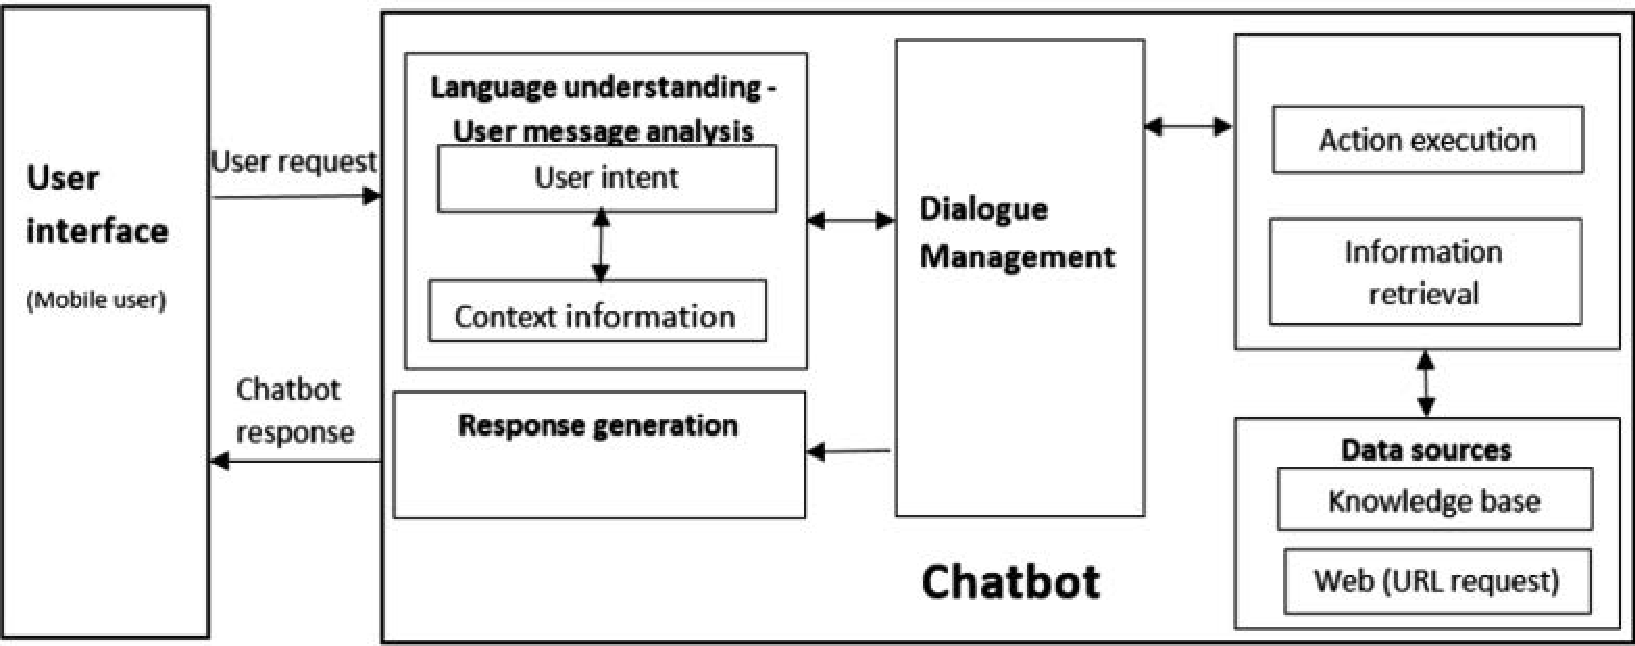
\includegraphics[width=12cm]{huang-arquitetura.pdf}
\caption{Arquitetura de um \textit{chatbot} segundo Huang et al. \cite{huang2021}.}
\label{fig:bot-arch}
\end{figure}

\section{Classificações de \textit{Bots}} \label{sec:class-bots}

Existem diversas formas de classificar \textit{bots}, dependendo de suas
características, funcionalidades e aplicações. Os \textit{bots} podem ser
classificados de acordo com seu propósito principal \cite{lebeuf2019}, ou de
acordo com a sua funcionalidade primária \cite{seering2018}.

\begin{table}[H]
\centering
\label{tab:classificacao_bots}
\begin{tabular}{|p{4.2cm}|p{9cm}|}
\hline
\textbf{Propósito}\cite{lebeuf2019}& \textbf{Descrição} \\
\hline
\textit{Bots} generalistas & Executam uma ampla variedade de tarefas, como
responder perguntas gerais e executar comandos simples. \\
\hline
\textit{Bots} transacionais & Realizam transações com sistemas externos, como
\textit{bots} bancários ou de compras. \\
\hline
\textit{Bots} informacionais & Fornecem informações e respondem perguntas
específicas dos usuários. \\
\hline
\textit{Bots} de produtividade & Automatizam tarefas repetitivas, como lembretes
ou agendamentos. \\
\hline
\textit{Bots} de colaboração & Facilitam a interação e colaboração entre
usuários, geralmente em ambientes de comunicação. \\
\hline
\hline
\textbf{Funcionalidade}\cite{seering2018} & \textbf{Descrição} \\
\hline
Tarefas administrativas & Auxiliam na organização de atividades, como agendar
reuniões e gerenciar compromissos. \\
\hline
Entretenimento & Proporcionam atividades lúdicas, como jogos ou interações
divertidas. \\
\hline
Funcionalidade e qualidade & Aumentam a eficiência de serviços, como
\textit{bots} de suporte técnico ou de coleta de \textit{feedback}. \\
\hline
Comunidade & Moderam e gerenciam interações em comunidades \textit{online}. \\
\hline
Arquivadores & Organizam e recuperam informações, como documentos e registros de
mensagens. \\
\hline
\end{tabular}
\caption{Classificação de \textit{bots} segundo propósito e funcionalidade}
\end{table}

\noindent Este trabalho concentra-se em \textit{bots} do tipo ``produtividade'' e
``colaboração'' como propósito, e ``funcionalidade e qualidade'' como
funcionalidade. O foco é a sua aplicação dentro do contexto educacional, onde
eles podem atuar como assistentes virtuais que facilitam a interação entre
alunos e professores, a fim de promover um ambiente remoto de aprendizagem mais
dinâmico e interativo.

\section{\textit{Bots} no Contexto Educacional} \label{sec:bots-educ}

Na educação, os \textit{bots} têm sido utilizados para diversos propósitos,
desde fornecer suporte administrativo até oferecer experiências de aprendizado
personalizadas. Os \textit{bots} educacionais podem transformar a experiência de
aprendizagem ao oferecer suporte contínuo e personalizado que seria impraticável
para um professor humano fornecer a todos os alunos simultaneamente
\cite{zawacki2019}.

Estudos recentes têm explorado aplicações educacionais específicas de
\textit{bots}. Por exemplo, o uso de \textit{chatbots} para melhorar a retenção
de conhecimento em estudantes universitários \cite{okonkwo2021}, e aumentar o
engajamento em cursos \textit{online} abertos e massivos (\textit{MOOCs})
\cite{han2022}.

De uma maneira geral, \textit{bots} educacionais são particularmente eficazes
quando (1) fornecem \textit{feedback} imediato aos alunos, (2) oferecem
disponibilidade contínua para assistência, (3) personalizam a experiência de
aprendizado, (4) reduzem a carga cognitiva dos instrutores e (5) permitem que os
instrutores se concentrem em atividades pedagógicas e interativas
\cite{silva2024}.

A seguir, exploramos quatro dimensões importantes relacionadas ao uso de
\textit{bots} educacionais: a Seção \ref{subsec:desafios} apresenta os desafios
específicos do ensino remoto que podem ser mitigados por essas ferramentas, a
Seção \ref{subsec:ihc} discute os princípios de interação humano-computador
relevantes para o \textit{design} de \textit{bots} educacionais eficazes, a
Seção \ref{subsec:principios} delineia os princípios fundamentais para a
interação mediada por \textit{bots} na educação, e finalmente, a Seção
\ref{subsec:dashboards} analisa o papel dos \textit{dashboards} como ferramentas
de controle pedagógico.

\subsection{Desafios do Ensino Remoto} \label{subsec:desafios}

O ensino remoto apresenta desafios únicos que podem ser parcialmente mitigados
pelo uso de tecnologias interativas como \textit{bots}. Aqui se faz distinção entre
``ensino remoto emergencial'' e educação \textit{online} planejada, destacando que
muitas instituições foram forçadas a adotar o primeiro modelo durante a pandemia
de COVID-19, sem tempo adequado para planejamento
\cite{hodges2020,fabiane2024}.

\noindent Entre os principais desafios identificados estão \cite{fabiane2024}:

\begin{itemize}
\item Limitações tecnológicas e acesso desigual
\item Competências digitais insuficientes de professores e alunos
\item Falta de estrutura para avaliação eficaz
\item Dificuldade em manter o engajamento dos alunos
\item Ausência de interação social e senso de comunidade
\end{itemize}

\noindent Tecnologias como \textit{bots} podem preencher algumas dessas lacunas
ao proporcionar uma interface natural e contínua entre os participantes do
processo educacional, oferecendo um canal adicional de comunicação e suporte
tanto para alunos quanto para professores \cite{winkler2018}.

\subsection{Interação Humano-Computador na Educação} \label{subsec:ihc}

Estudos em IHC destacam a importância de sistemas que se ajustem ao
comportamento e às necessidades dos usuários \cite{roy1987}. Na educação, isso
implica em promover interfaces que permitam participação ativa, acessibilidade e
adaptabilidade aos estilos de aprendizagem dos alunos.

Norman \cite{norman2013} enfatiza o conceito de \textit{design} centrado no
usuário, onde a tecnologia deve se adaptar às necessidades humanas e não o
contrário. Aplicado ao contexto educacional, este princípio sugere que os
\textit{bots} devem ser projetados considerando as necessidades pedagógicas
específicas e as limitações cognitivas dos alunos.

\textit{Bots} educacionais se encaixam nesse contexto por serem acessíveis e
flexíveis na forma de interação. Interfaces conversacionais podem reduzir a
carga cognitiva associada à navegação em sistemas educacionais complexos,
permitindo que os alunos se concentrem no conteúdo do aprendizado em vez de na
interface \cite{sweller2011}.

\subsection{Princípios para Interação Mediada por \textit{Bots} na Educação}
\label{subsec:principios}

Com base na literatura sobre \textit{bots} educacionais e metodologias ativas,
surgem três princípios fundamentais emergem como pilares para o \textit{design}
de interações eficazes mediadas por \textit{bots} em ambientes educacionais:

\begin{enumerate}
\item \textbf{Comunicação multidirecional}: Um \textit{bot} educacional eficaz
não deve apenas transmitir informações do professor para os alunos, mas também
facilitar o retorno dos alunos para o professor, criando um ciclo contínuo de
\textit{feedback}.  Esse princípio alinha-se com a concepção de aprendizagem
dialógica
\cite{calvo2013}, onde o conhecimento é construído através da interação
bidirecional entre educador e educando.
\item \textbf{Engajamento ativo}: Através de mecânicas interativas, o
\textit{bot} deve estimular constantemente a participação dos alunos,
transformando-os de receptores passivos a agentes ativos no processo de
aprendizagem. Este princípio está fundamentado nas teorias construtivistas de
aprendizagem \cite{piaget1970}, que enfatizam a importância da experiência
prática e da participação na construção do conhecimento.
\item \textbf{Adaptação contextual}: O sistema deve se ajustar ao ritmo da aula
e às necessidades específicas da disciplina, oferecendo diferentes modos de
interação conforme o momento pedagógico. Tecnologias educacionais eficazes devem
ser flexíveis o suficiente para se adaptarem a diferentes contextos pedagógicos
e estilos de aprendizagem \cite{winkler2018}.
\end{enumerate}

Estes princípios fornecem uma base teórica para o \textit{design} de
\textit{bots} educacionais que efetivamente aprimoram o processo de
aprendizagem, especialmente em contextos de metodologias ativas onde a
participação e o engajamento dos alunos são essenciais.

\subsection{\textit{Dashboards} como Ferramenta de Controle Pedagógico}
\label{subsec:dashboards}

Um elemento crucial no \textit{design} de \textit{bots} educacionais é a
interface de controle que permite aos educadores gerenciar o fluxo das
interações. Os \textit{dashboards} pedagógicos surgem como uma solução para esta
necessidade, oferecendo uma visão consolidada das atividades e permitindo
intervenções em tempo real sem interromper o fluxo da aula \cite{verbert2013}.

\textit{Dashboards} de aprendizagem são ``\textit{displays} únicos que agregam
diferentes indicadores sobre aprendiz, atividades de aprendizagem e/ou contexto
de aprendizagem em uma ou múltiplas visualizações'' \cite{verbert2013}. No
contexto de \textit{bots} educacionais, estes \textit{dashboards} evoluem para
se tornarem não apenas ferramentas de visualização, mas interfaces de comando
que permitem aos professores:

\begin{enumerate}
\item \textbf{Orquestrar atividades}: Iniciar e controlar sequências de
aprendizagem sem necessidade de inserir comandos em \textit{chats} públicos
\item \textbf{Monitorar em tempo real}: Visualizar métricas de engajamento e
compreensão durante a aula
\item \textbf{Receber alertas}: Ser notificado sobre padrões que exijam
intervenção pedagógica
\item \textbf{Personalizar interações}: Adaptar atividades com base nas
necessidades observadas
\item \textbf{Analisar resultados}: Obter relatórios detalhados após as sessões
\end{enumerate}

\begin{figure}[H] \centering
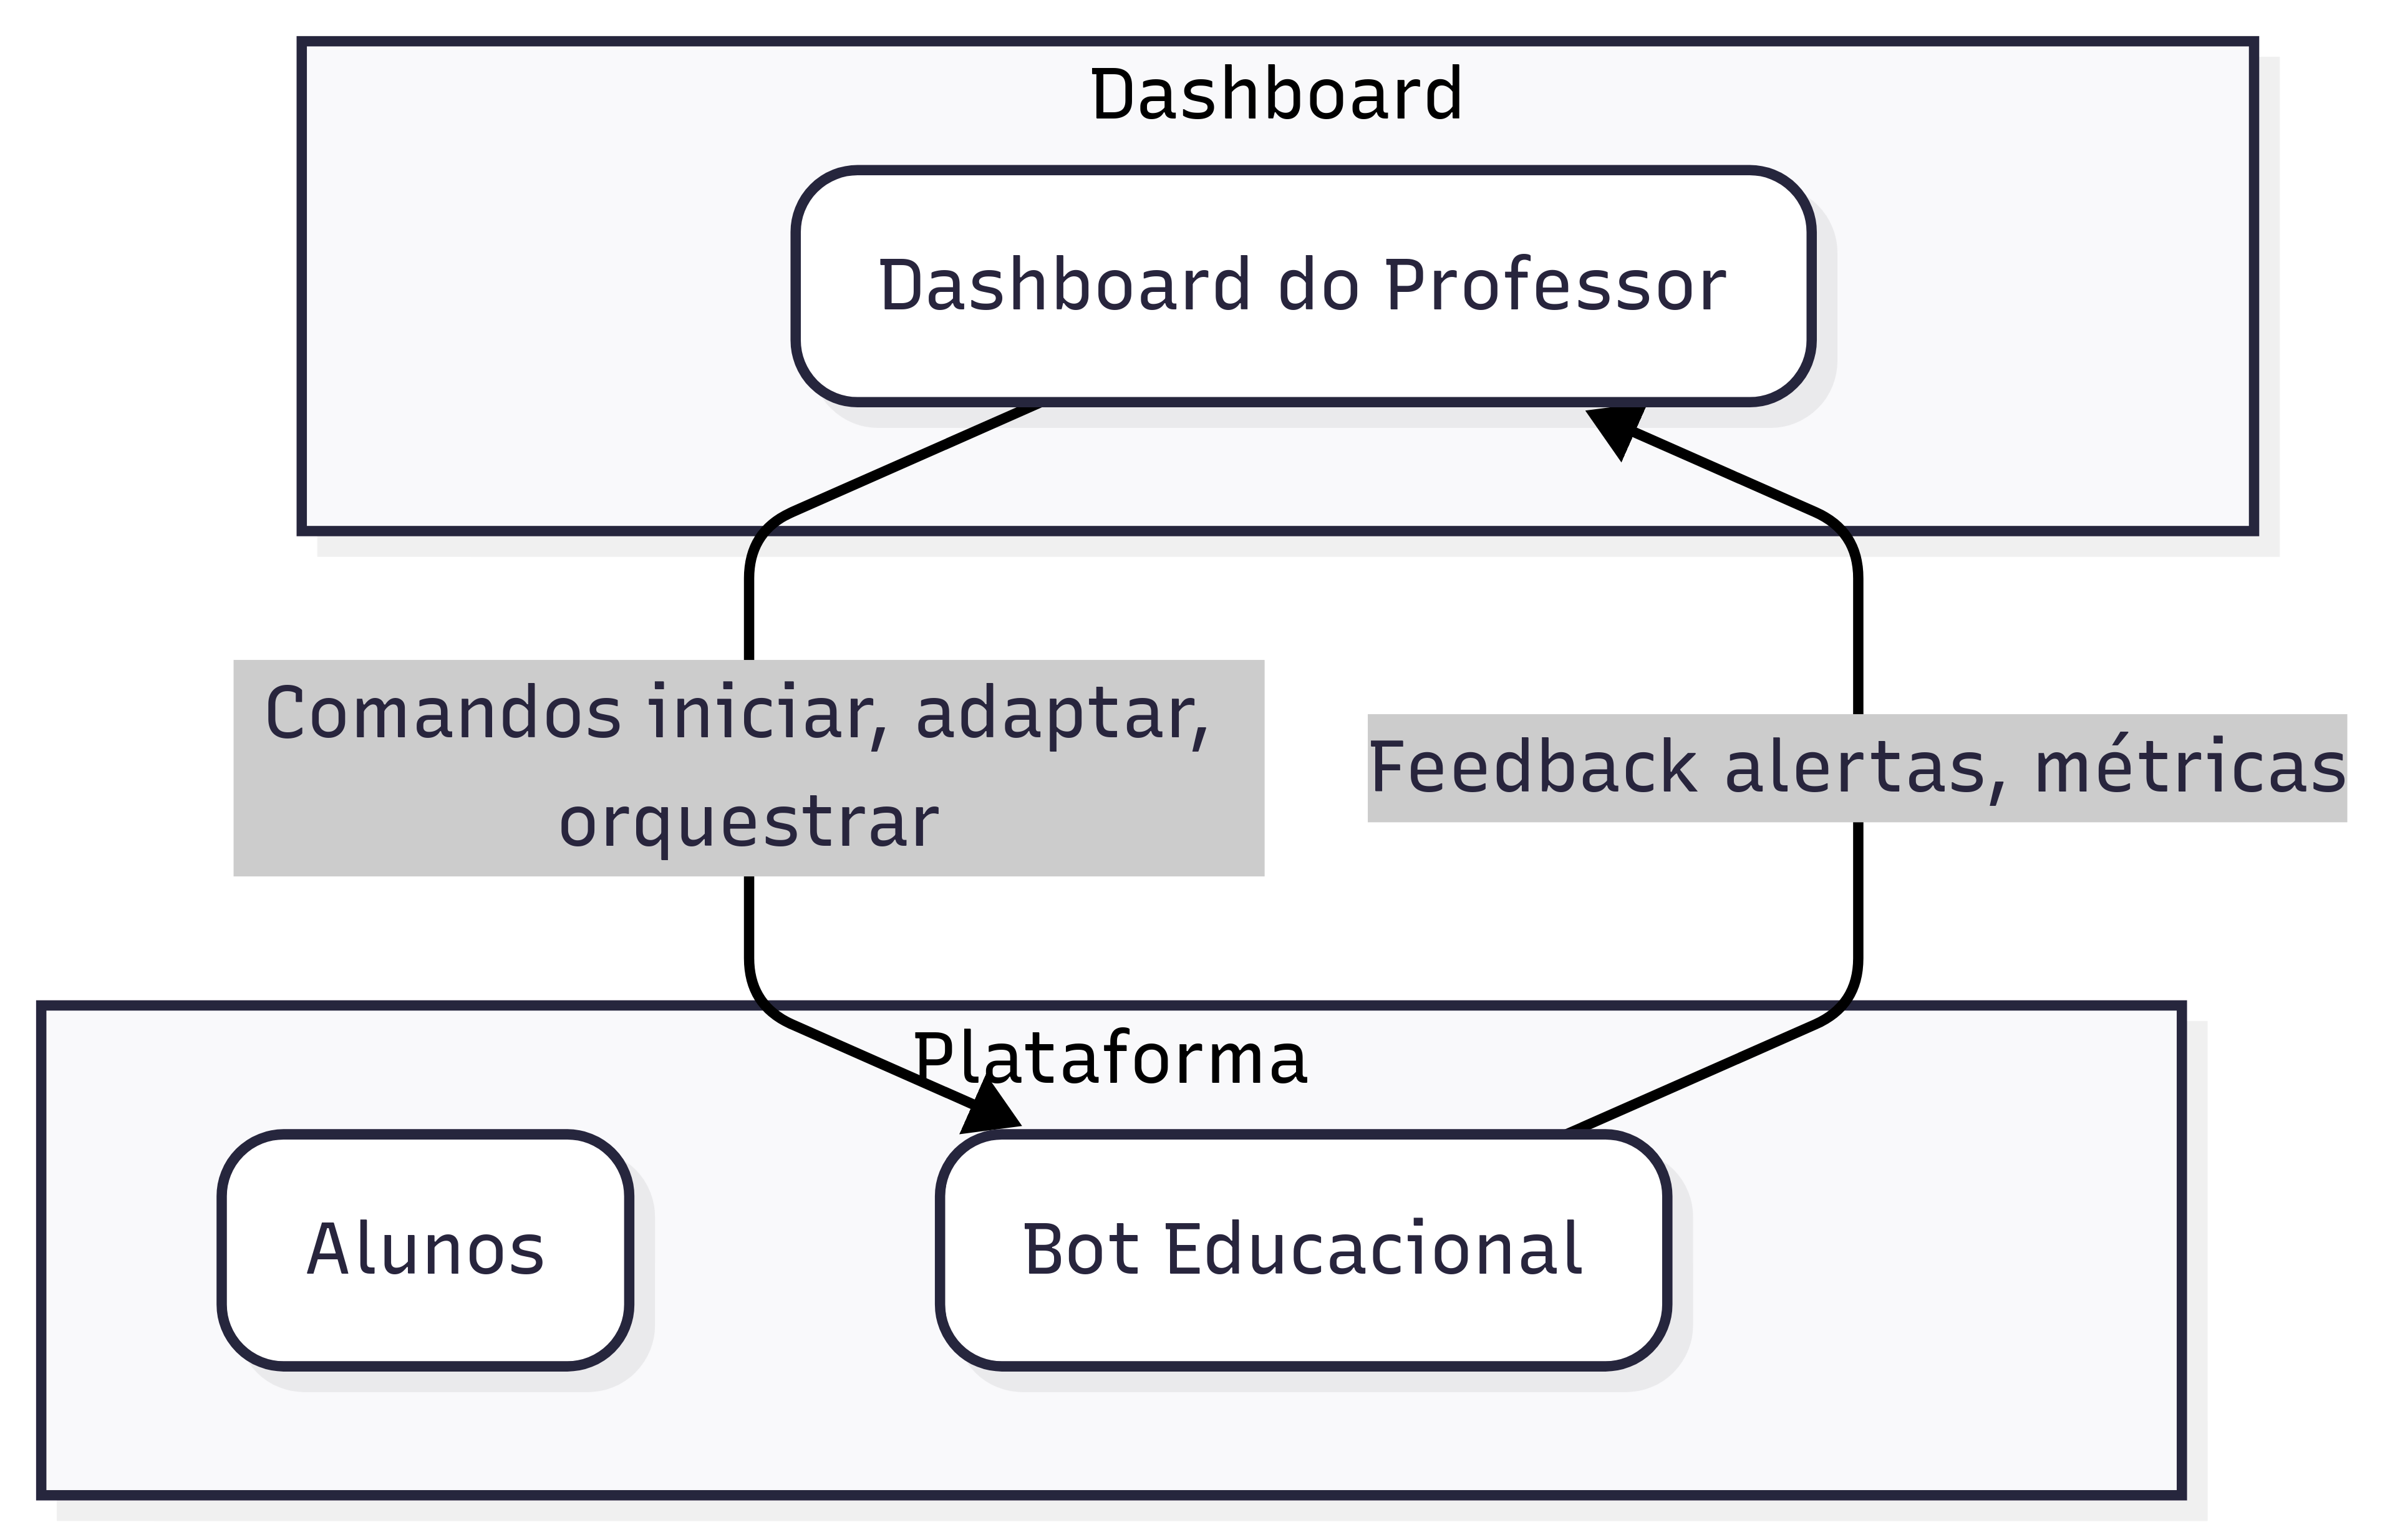
\includegraphics[width=12cm]{relacao-dashboard-bot.png}
\caption{Relação entre o \textit{bot} educacional e o \textit{dashboard} de
controle pedagógico.}
\label{fig:dashboard-bot}
\end{figure}

Esta abordagem separa claramente o canal de comando (\textit{dashboard}, visível
apenas para o professor) do canal de interação (plataforma de comunicação,
visível para todos os participantes), seguindo o princípio de ``separação de
interesses'' \cite{huang2021} como essencial para ambientes de aprendizagem
tecnologicamente mediados. A eficácia desse modelo de interação será avaliada em
experimentos controlados, onde participantes assumirão papéis de professor e
alunos, interagindo em um ambiente de sala de aula simulado.

\section{Ferramentas para Desenvolvimento de \textit{Bots} no Discord}
\label{sec:ferramentas}

Existem várias plataformas que permitem desenvolver \textit{bots} educacionais,
como por exemplo, no Moodle, que é uma plataforma de gestão de aprendizagem
amplamente utilizada em ambientes educacionais \cite{pietrusky2024chatbot}, e
também no Slack, que é uma plataforma de comunicação corporativa que também pode
ser utilizada para fins educacionais \cite{wright2024enhancing}. Dentre destas 
escolhemos o Discord, uma plataforma de comunicação digital que apesar de ter
sido originalmente desenvolvida para comunidades de jogos, apresenta as
seguintes características que a tornam adequada para emular um ambiente
educacional remoto \cite{espinoza2021}:

\begin{itemize}
\item \textbf{Comunicação em tempo real}: Permite interações síncronas e
assíncronas
\item \textbf{Canais temáticos}: Permitem organizar discussões por tópicos
específicos
\item \textbf{Transmissão de voz/vídeo}: Facilita aulas síncronas com interação
audiovisual
\item \textbf{Compartilhamento de tela}: Possibilita demonstrações práticas pelo
professor
\item \textbf{Sistema de reações}: Oferece mecanismo não-verbal para expressão
de compreensão ou dúvidas
\item \textbf{Persistência de mensagens}: Mantém o histórico de interações
disponível para consulta posterior
\end{itemize}

Sendo assim, destacamos algumas bibliotecas específicas para desenvolvimento de
\textit{bots} na plataforma do Discord, cada uma com suas particularidades e
casos de uso apropriados, (1) JavaScript/Node.js, (2) Python e (3) C.

\begin{enumerate}
\item \textbf{Discord.js}\cite{discordjs}: Uma biblioteca JavaScript/Node.js que
oferece abstração de alto nível para interação com a \textit{API} do Discord. É
rica em recursos e possui uma comunidade ativa, sendo adequada para
desenvolvedores que preferem desenvolvimento rápido.
\item \textbf{Discord.py}\cite{discordpy}: Equivalente ao Discord.js, mas para a
linguagem Python. Oferece abstrações semelhantes e é amplamente utilizada para
desenvolvimento de \textit{bots} no Discord.
\item \textbf{Concord}\cite{muller}: Uma biblioteca em C que fornece acesso de
baixo nível à \textit{API} do Discord, desenvolvida pelo autor deste trabalho
durante o período da pandemia de COVID-19, como um projeto \textit{hobby}.
Diferentemente das opções anteriores, a Concord prioriza desempenho e controle
direto sobre a \textit{API}, sendo apropriada para aplicações que demandam
eficiência computacional e controle granular.
\end{enumerate}

No contexto deste estudo, foi escolhida a biblioteca Concord, por sua
implementação na linguagem C, que oferece um equilíbrio entre abstração e
controle que a torna adequada para uma ampla gama de aplicações
\cite{kernighan1988}. E também pela familiaridade do autor com a biblioteca, que
facilita o desenvolvimento e a manutenção do \textit{bot} educacional proposto.

Para estudos futuros, é importante considerar o uso de linguagens de mais alto
nível como Python, JavaScript ou Go, que podem oferecer desenvolvimento mais
rápido e maior facilidade de manutenção para equipes maiores, especialmente em
projetos onde a curva de aprendizado reduzida seja prioritária em relação ao
desempenho bruto. A linguagem de programação em contextos educacionais deve
equilibrar considerações pedagógicas, praticidade de implementação e objetivos
específicos do projeto
\cite{pears2007}.

\section{Trabalhos Relacionados} \label{sec:trab-rel}

Diversos pesquisadores têm explorado o uso de \textit{bots} em contextos
educacionais:

Hien et al. \cite{hien2018} desenvolveram um \textit{bot} para suporte a alunos
em um curso de programação, que respondia a dúvidas sobre conceitos e sintaxe.
Os resultados mostraram uma redução no tempo de resposta para dúvidas comuns e
um aumento na satisfação dos alunos com o suporte recebido.

Demetriadis et al. \cite{demetriadis2018} implementaram um agente conversacional
para auxiliar alunos em atividades colaborativas de resolução de problemas. O
estudo demonstrou que grupos apoiados pelo \textit{bot} apresentaram maior
engajamento e melhores resultados de aprendizagem em comparação com grupos sem
suporte automatizado.

Yin et al. \cite{yin2024} compararam o fornecimento de \textit{feedback}
formativo aos alunos por \textit{chatbot} e professor. A avaliação indicou que
alunos que receberam \textit{feedback} regularmente do \textit{chatbot}
apresentaram maior interesse de aprendizagem, além de redução da carga cognitiva
necessária para aprender conceitos complexos.

Um trabalho particularmente relevante é o de Winkler e Söllner
\cite{winkler2018}, por propor diretrizes para o \textit{design} de
\textit{chatbots} educacionais focados em metodologias ativas, destacando a
importância de promover interações que estimulem o pensamento crítico e a
reflexão.

Os próximos capítulos detalham a concepção e implementação do \textit{bot} 
educacional proposto, bem como sua avaliação através da metodologia experimental
com participantes em diferentes papéis, demonstrando como os conceitos teóricos
discutidos neste capítulo se manifestam na prática educacional.
